%************************************************
\chapter{Teoria}\label{ch:teoria}
%************************************************
\section{Introduzione}

La TDA si prefigge come obiettivo quello di trovare strutture complesse in un insieme di dati. Finora sono stati conseguiti risultati come la determinazione di nuove variabili che influenzano l'attività neurale \cite{Spreemann2015}, la classificazione di traiettorie in robotica \cite{Pokorny2014}, l'identificazione di nuovi tipi di cancro al seno \cite{Lum2013}, e molti altri.

La novità della TDA sta nel provare a catturare la \emph{forma} dei dati e, in questa, cercare proprietà topologiche interessanti che costituiscano un segnale anziché un rumore.

\begin{figure}
  \begin{center}
    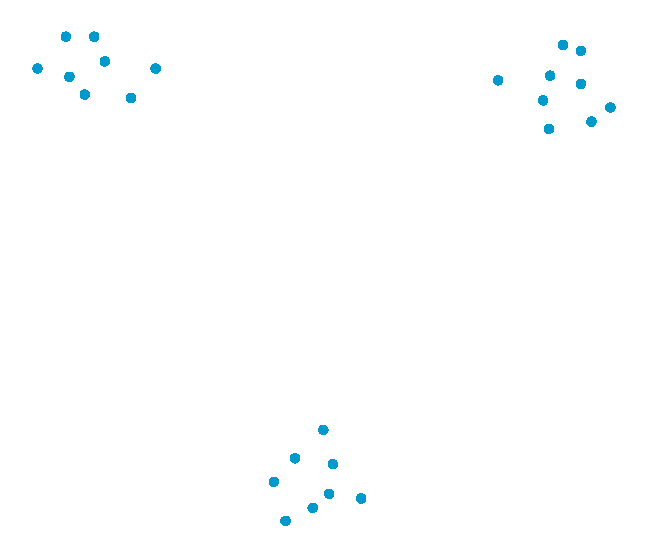
\includegraphics[width=.4\linewidth]{gfx/three_clusters_small.pdf}
    \caption{Dati divisi in più cluster}
    \label{fig:clusters}
  \end{center}
\end{figure}

Ad esempio, consideriamo un insieme di dati come in \cref{fig:clusters}. È chiaro a chi osserva che vi sono tre gruppi di punti, tuttavia la formalizzazione matematica di questa osservazione non è immediata.

Un modo potrebbe essere il seguente: sia
\begin{equation*}
  X=\{x_1,\dots, x_n\}
\end{equation*}
il nostro insieme di dati, consideriamo per $\varepsilon>0$ l'insieme
\begin{equation*}
  \hat{X}_\varepsilon=\cup_{0\leq i\leq n} B(x_i,\varepsilon)
\end{equation*}
where $B(x_i,\varepsilon)$ è la palla di centro $x_i$ e raggio $\varepsilon$. Osserviamo che esiste un intervallo di valori $a \leq \varepsilon \leq b$ per cui $\hat{X}_\varepsilon$ appare come in \cref{fig:clusters_fat}.

\begin{figure}
  \begin{center}
    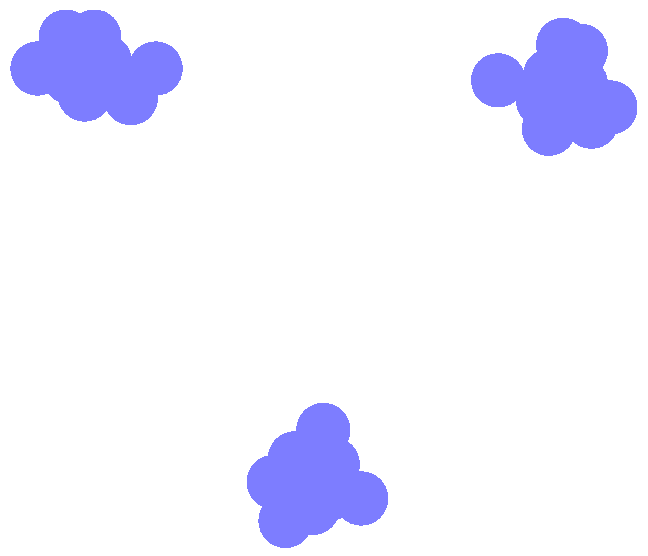
\includegraphics[width=.4\linewidth]{gfx/three_clusters_fat.pdf}
    \caption{$\hat{X}_\varepsilon$}
    \label{fig:clusters_fat}
  \end{center}
\end{figure}

Allora possiamo possiamo calcolare il numero di componenti connesse, o equivalentemente la dimensione del gruppo di omologia $\H{0}(\hat{X}_\varepsilon;k)=k^3$, dove $k$ è un campo,
